%-------------------------
% Resume in Latex
% Author
% License : MIT
%------------------------

%---- Required Packages and Functions ----

\documentclass[a4paper,11pt]{article}
\usepackage{latexsym}
\usepackage{xcolor}
\usepackage{float}
\usepackage{ragged2e}
\usepackage[empty]{fullpage}
\usepackage{wrapfig}
\usepackage{lipsum}
\usepackage{tabularx}
\usepackage{titlesec}
\usepackage{geometry}
\usepackage{marvosym}
\usepackage{verbatim}
\usepackage{enumitem}
\usepackage[hidelinks]{hyperref}
\usepackage{fancyhdr}
\usepackage{fontawesome5}
\usepackage{multicol}
\usepackage{graphicx}
\usepackage{cfr-lm}
\usepackage[T1]{fontenc}
\setlength{\multicolsep}{0pt} 
\pagestyle{fancy}
\fancyhf{} % clear all header and footer fields
\fancyfoot{}
\renewcommand{\headrulewidth}{0pt}
\renewcommand{\footrulewidth}{0pt}
\geometry{left=1.4cm, top=0.8cm, right=1.2cm, bottom=1cm}
% Adjust margins
%\addtolength{\oddsidemargin}{-0.5in}
%\addtolength{\evensidemargin}{-0.5in}
%\addtolength{\textwidth}{1in}
\usepackage[most]{tcolorbox}
\tcbset{
	frame code={}
	center title,
	left=0pt,
	right=0pt,
	top=0pt,
	bottom=0pt,
	colback=gray!20,
	colframe=white,
	width=\dimexpr\textwidth\relax,
	enlarge left by=-2mm,
	boxsep=4pt,
	arc=0pt,outer arc=0pt,
}

\urlstyle{same}

\raggedright
\setlength{\tabcolsep}{0in}

% Sections formatting
\titleformat{\section}{
  \vspace{-4pt}\scshape\raggedright\large
}{}{0em}{}[\color{black}\titlerule \vspace{-7pt}]

%-------------------------
% Custom commands
\newcommand{\resumeItem}[2]{
  \item{
    \textbf{#1}{\hspace{0.5mm}#2 \vspace{-0.5mm}}
  }
}

\newcommand{\resumePOR}[3]{
\vspace{0.5mm}\item
    \begin{tabular*}{0.97\textwidth}[t]{l@{\extracolsep{\fill}}r}
        \textbf{#1}\hspace{0.3mm}#2 & \textit{\small{#3}} 
    \end{tabular*}
    \vspace{-2mm}
}

\newcommand{\resumeSubheading}[4]{
\vspace{0.5mm}\item
    \begin{tabular*}{0.98\textwidth}[t]{l@{\extracolsep{\fill}}r}
        \textbf{#1} & \textit{\footnotesize{#4}} \\
        \textit{\footnotesize{#3}} &  \footnotesize{#2}\\
    \end{tabular*}
    \vspace{-2.4mm}
}

\newcommand{\resumeProject}[4]{
\vspace{0.5mm}\item
    \begin{tabular*}{0.98\textwidth}[t]{l@{\extracolsep{\fill}}r}
        \textbf{#1} & \textit{\footnotesize{#3}} \\
        \footnotesize{\textit{#2}} & \footnotesize{#4}
    \end{tabular*}
    \vspace{-2.4mm}
}

\newcommand{\resumeSubItem}[2]{\resumeItem{#1}{#2}\vspace{-4pt}}

% \renewcommand{\labelitemii}{$\circ$}
\renewcommand{\labelitemi}{$\vcenter{\hbox{\tiny$\bullet$}}$}

\newcommand{\resumeSubHeadingListStart}{\begin{itemize}[leftmargin=*,labelsep=0mm]}
\newcommand{\resumeHeadingSkillStart}{\begin{itemize}[leftmargin=*,itemsep=1.7mm, rightmargin=2ex]}
\newcommand{\resumeItemListStart}{\begin{justify}\begin{itemize}[leftmargin=3ex, rightmargin=2ex, noitemsep,labelsep=1.2mm,itemsep=0mm]\small}

\newcommand{\resumeSubHeadingListEnd}{\end{itemize}\vspace{2mm}}
\newcommand{\resumeHeadingSkillEnd}{\end{itemize}\vspace{-2mm}}
\newcommand{\resumeItemListEnd}{\end{itemize}\end{justify}\vspace{-2mm}}
\newcommand{\cvsection}[1]{%
\vspace{2mm}
\begin{tcolorbox}
    \textbf{\large #1}
\end{tcolorbox}
    \vspace{-4mm}
}

\newcolumntype{L}{>{\raggedright\arraybackslash}X}%
\newcolumntype{R}{>{\raggedleft\arraybackslash}X}%
\newcolumntype{C}{>{\centering\arraybackslash}X}%
%---- End of Packages and Functions ------

%-------------------------------------------
%%%%%%  CV STARTS HERE  %%%%%%%%%%%
%%%%%% DEFINE ELEMENTS HERE %%%%%%%
\newcommand{\name}{Prathamesh Sabale} % Your Name
\newcommand{\course}{B.Tech} % Your Program
\newcommand{\roll}{xxxxxxx} % Your Roll No.
\newcommand{\phone}{xxxxxxxxxx} % Your Phone Number
\newcommand{\emaila}{youremail@email.com} %Email 1





\begin{document}
\fontfamily{cmr}\selectfont
%----------HEADING-----------------


\parbox{2.35cm}{%
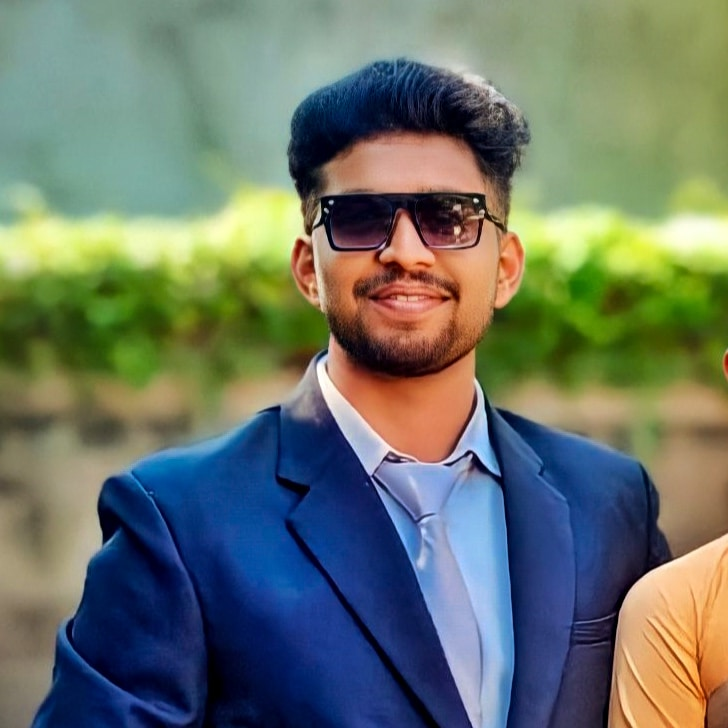
\includegraphics[width=2cm,clip]{my.jpg}
}
\parbox{\dimexpr\linewidth-2.8cm\relax}{
\begin{tabularx}{\linewidth}{L r} \\
  \textbf{\Large \name} & {\raisebox{0.0\height}{\footnotesize \faPhone}\ +91 9881791672}\\
  {Roll No.: 20141216} & \href{mailto:\emaila}{\raisebox{0.0\height}{\footnotesize \faEnvelope}\ {prathamms07@gmail.com}} \\
  {Information Technology} &  \href{https://github.com/prathamms07}{\raisebox{0.0\height}{\footnotesize \faGithub}\ {prathamms07}} \\
  {Government College Of Engineering Karad} & \href{www.linkedin.com/in/prathamesh-sabale-422291209}{\raisebox{0.0\height}{\footnotesize \faLinkedin}\ {Prathamesh Sabale}}
\end{tabularx}
}
% \parbox{3.0cm}{%
% \flushright \includegraphics[width=2cm,clip]{nitp_logo.png}
% }




%-----------EDUCATION-----------
\section{\textbf{Education}}
  \resumeSubHeadingListStart
    \resumeSubheading
      {Government College of Engineering, Karad}{CGPA:8.5}
      {Bachelor of Technology, Information Technology}{2024}
    \resumeSubheading
      {Jawahar Navodaya Vidyalaya}{Percentage:76}
      {Central Board for Secondary Education, Class 12th}{2020}
    \resumeSubheading
      {De Paul English Medium High School}{Percentage:89}
      {Maharashtra State Board, Class 10th}{2018}
  \resumeSubHeadingListEnd
\vspace{-5.5mm}
%



%-----------EXPERIENCE-----------------
\section{\textbf{Internships}}
  \resumeSubHeadingListStart
    \resumeSubheading
      {Object Oriented Programming And DSA}
      {July-August,2021}{Zenox Technologies}
      
    
    
    \vspace{-1.0mm}
    
    \resumeSubheading
      {Amazon Web Services}{June-July,2022}
      {Sensix InfoTech}{}
      \vspace{-2.0mm}
      
\vspace{-0.0mm}



%-----------PROJECTS-----------------
\section{\textbf{Projects}}
\resumeSubHeadingListStart

    \resumeProject
      {Object Detection With OpenCV} %Project Name
      {The primary aim behind this project was to have hands-on experience while learning Computer Vision} %Project Name, Location Name
     

      \resumeItemListStart
        \item {Tools \& technologies used: Computer Vision, Image Processing}
        \item { Project predicts object name with percentage accuracy of predicted class being true.}
    \resumeItemListEnd
    \vspace{-1mm}
    
    \resumeProject
      {Dairy Management System} %Project Name
      {The aim was to use oops concepts to build a program to keep track of dairy activities like record maintenance and billing.} %Project Name, Location Name
      

      \resumeItemListStart
        \item {Tools \& technologies used: OOPs with C++}
        \item {It program kept the track of current stock of milk and amount of milk delivered by each customer. }
    \resumeItemListEnd
    \vspace{-2mm}
    
      
  \resumeSubHeadingListEnd
\vspace{-5.5mm}



%-----------Technical skills-----------------
\section{\textbf{Technical Skills and Interests}}
 \begin{itemize}[leftmargin=0.05in, label={}]
    \small{\item{
     \textbf{Languages}{: C , C++, Python, Java} \\
  \textbf{Tools}{: Github, Power BI, Kali Linux} \\
     \textbf{Cloud & Databases}{: Amazon Web Services , MySQL } \\
     \textbf{Soft Skills}{: Adaptability, Leadership, Teamwork } \\
     \textbf{Coursework}{: Computer Networking, Database Management System, SSOS, Object Oriented Programming, IOT } \\
     \textbf{Areas of Interest}{:  Artificial Intelligence and Machine Learning , Ethical Hacking} \\  \textbf{Other Projects }{:  ChatBot, Hospital Website, Launcing Webiste with AWS, Automated Light System} \\

     \end{itemize}
 \vspace{-2.5mm}



%-----------Positions of Responsibility-----------------
\section{\textbf{Positions of Responsibility}}
\vspace{-0.4mm}
\resumeSubHeadingListStart
\resumePOR{President, } % Position
    {Artificial Intelligence and Computer Vision Club} %Club,Event
    {2022 to Present} %Tenure Period
\resumePOR{Joint Secretary, } % Position
    {Information Technology Students Association} %Club,Event
    {Present} %Tenure Period
    \resumePOR{Class Representative } % Position
    {} %Club,Event
    {FY to Present} %Tenure Period
    \resumePOR{Event Management Team, } % Position
    {AlphaGeeks Club} %Club,Event
    {2022-Present} %Tenure Period
\resumeSubHeadingListEnd
\vspace{-5mm}




%-----------Achievements-----------------
\section{\textbf{Certifications}}
\vspace{-0.4mm}
\resumeSubHeadingListStart
\resumePOR{Python-Introduction to Data Science and Machine Learning A-Z  } % Award
    {} % Event
    {Oct 2022} %Event Year
    
\resumePOR{Technical Support Fundamentals, by Google } % Award
    {} % Event
    {Dec 2022} %Event Year
\resumePOR{Bits and Bytes of Computer Networking, by Google } % Award
    
    {Feb 2023 } %Event Year
\resumePOR{Complete Core Java Course} % Award
    
    {June 2023} %Event Year
    
\resumeSubHeadingListEnd
\vspace{-5mm}



%-------------------------------------------
%-----------Achievements-----------------
\section{\textbf{Achievements}}
\vspace{-0.4mm}
\resumeSubHeadingListStart

    
\resumePOR{Secured Third Rank in Ideathon  } % Award
    {} % Event
    {January 2023} %Event Year

    \resumePOR{ Finalist in  Technovation } % Award
    {} % Event
    {March 2023} %Event Year

     \resumePOR{ Second position, Judo Regional } % Award
    {} % Event
    {September 2020} %Event Year
\resumeSubHeadingListEnd
\vspace{-5mm}



%-------------------------------------------
\end{document}
